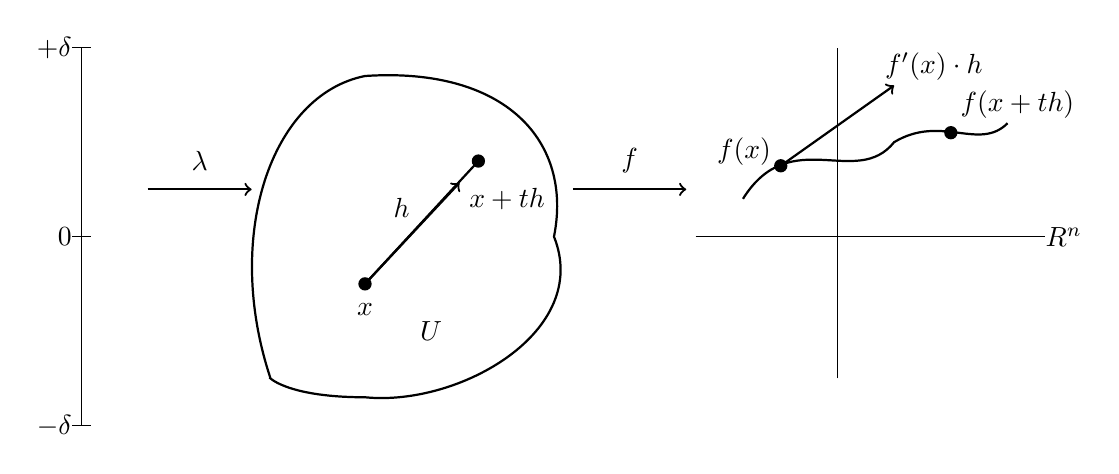
\begin{tikzpicture}[scale=1.2]

% ---- Intervalo (-eps, eps)
\draw (-4,-2) -- (-4,2);
\draw (-4.1,2) -- (-3.9,2);
\draw (-4.1,-2) -- (-3.9,-2);
\draw (-4.1,0) -- (-3.9,0);

\node[left] at (-4,2) {$+\delta$};
\node[left] at (-4,0) {$0$};
\node[left] at (-4,-2) {$-\delta$};

% flecha \lambda
\draw[->, thick] (-3.3,0.5) -- (-2.2,0.5);
\node at (-2.75,0.8) {$\lambda$};

% ---- Conjunto U
\draw[thick]
(-2,-1.5) .. controls (-2.5,0) and (-2,1.5) ..
(-1,1.7) .. controls (0.5,1.8) and (1.2,1) ..
(1,0) .. controls (1.4,-1) and (0,-1.8) ..
(-1,-1.7) .. controls (-1.8,-1.7) and (-2,-1.5) ..
cycle;

\node at (-0.3,-1.0) {$U$};

% punto x
\fill (-1, -0.5) circle (2pt);
\node[below] at (-1,-0.6) {$x$};

% flecha h
\draw[->,thick] (-1,-0.5) -- (0,0.57);
\node[right] at (-0.8,0.3) {$h$};

% punto x+th
\fill (0.2,0.8) circle (2pt);
\node[right] at (0,0.4) {$x+th$};

% vector h
\draw[-, thick] (-1,-0.5) -- (0.2,0.8);

% flecha f
\draw[->, thick] (1.2,0.5) -- (2.4,0.5);
\node at (1.8,0.8) {$f$};

% ---- grafica en R^n
\begin{scope}[shift={(4,0)}]

\draw (-1.5,0) -- (2.2,0);
\draw (0,-1.5) -- (0,2);

\node[right] at (2.1,0) {$\mathbb{R}^n$};

% curva
\draw[thick]
(-1,0.4) .. controls (-0.5,1.2) and (0.2,0.5) ..
(0.6,1) .. controls (1.1,1.3) and (1.5,0.9) ..
(1.8,1.2);

% punto f(x)
\fill (-0.6,0.75) circle (2pt);
\node[left] at (-0.6,0.9) {$f(x)$};

% punto f(x+th)
\fill (1.2,1.1) circle (2pt);
\node[right] at (1.2,1.4) {$f(x+th)$};

% vector derivada
\draw[->, thick] (-0.6,0.75) -- (0.6,1.6);
\node[right] at (0.4,1.8) {$f'(x)\cdot h$};

\end{scope}

\end{tikzpicture}
